\PassOptionsToPackage{unicode}{hyperref}
\documentclass[aspectratio=1610, 9pt]{beamer}

% Load packages you need here
\usepackage{polyglossia}
\setmainlanguage{english}

\usepackage{csquotes}
    

\usepackage{amsmath}
\usepackage{amssymb}
\usepackage{mathtools}

\usepackage{hyperref}
\usepackage{bookmark}
\usepackage[
  locale=UK,
  separate-uncertainty=true,
  per-mode=symbol-or-fraction,
]{siunitx}
\usepackage[
  backend=biber,   % use modern biber backend
  autolang=hyphen, % load hyphenation rules for if language of bibentry is not
  % german, has to be loaded with \setotherlanguages
  % in the references.bib use langid={en} for english sources
  sorting=none,
  ]{biblatex}
  \addbibresource{references.bib}  % the bib file to use
  \DefineBibliographyStrings{english}{andothers = {{et\,al\adddot}}}  % replace u.a. with et al.
  
  
% load the theme after all packages
\usetheme[
  showtotalframes, % show total number of frames in the footline
]{tudo}

% Put settings here, like
\unimathsetup{
  math-style=ISO,
  bold-style=ISO,
  nabla=upright,
  partial=upright,
  mathrm=sym,
}
\setbeamertemplate{caption}{\raggedright\insertcaption\par}

\title{Determining the dielectric function through THz-Transmission measurments}
\author[M.~Koch]{Max Koch}
\institute[AG Wang]{Arbeitsgruppe Wang \\  Fakultät Physik}
%\titlegraphic{\includegraphics[width=0.3\textwidth, angle=90]{images/setup.jpeg}}


\begin{document}

\maketitle

\section{Goal}
\begin{frame}
The First goal is to determine the refractive index 
\begin{equation}
  n_s = n - i\kappa
\end{equation}
which contains the real part $n$ nad complex part $\kappa$ of the refractive index.
\end{frame}

\section{Scheme}
\begin{frame}{Scheme}
  Lets first take a look at the experimental scheme
  \begin{center}
  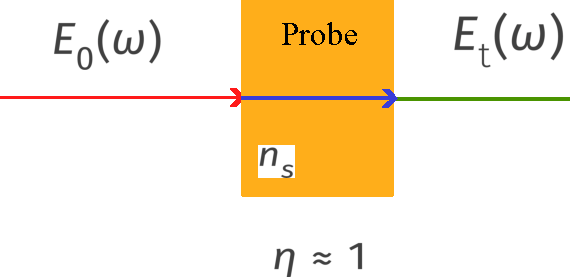
\includegraphics[width=0.5\textwidth]{images/Transmission.pdf}
  \end{center}
  The incoming THz-pulse $E_0(\omega)$ gets diffracted two times, indicated by the arrows, before it leaves the probe as the transmitted wave $E_\text{t}(\omega)$.
  For simplicity sake it is easier to assume an incident angel of $\theta=\SI{0}{\degree}$.
  All reflections are neglected.
  As defined earlier the probe has the refractive index $n_s$, its length is set to be $l$.
  The refractive index of the surrounding medium is $\eta$ in case of air $\eta\approx 1$.
\end{frame}

\begin{frame}{Transmitted wave}
  The transmitted wave is defined as 
  \begin{equation}
    E_\text{t}(\omega) = t(\omega) E_0(\omega)
  \end{equation}
  where
  \begin{equation}
    t(\omega) = \tau \tau' \symup{exp}\left[- i n_s(\omega) \frac{\omega l }{c}\right]
  \end{equation}
  is the transmission coeffiecient.
  The transmission coeffiecient is derived from the fresnel equations.
  Basically the wave is defracted two times, once when entering the medium and one when leaving the medium hence $\tau$ and $\tau'$.
  The defraction also generates a phase difference, which is represented by the exponential function.
  The complex transmission coeffiecients 
  \begin{align}
    \tau = & \frac{2}{1 + n_s} \\
    \tau' = &  \frac{2 n_s}{1+ n_s} 
  \end{align}
  are dependent on the refractive index $n_s$.
\end{frame}

\begin{frame}
  Lets do a first summary of our assumptions so far:
  \begin{itemize}
    \item No reflections
    \item Incident angle of $\theta=\SI{0}{\degree}$
    \item The probe is completly homogenous
  \end{itemize}
  with those assumptions the transmitted wave can be written as 
  \begin{equation}
    E_\text{t}(\omega) = \eta\frac{4 n_s (\omega)}{(n_s(\omega) + 1)^2} \symup{exp}\left[ -i n_s (\omega) \frac{\omega l }{c}\right] E_0(\omega)
  \end{equation}
\end{frame}

\begin{frame}{References measurment}
  To determine the refractive index it is necessary to know the properties of the uninterrupted THz-pulse.
  For this a references measurment of the THz-pulse is taken.
  The references wave 
  \begin{equation}
  E_\text{ref}(\omega) = \eta \symup{exp}\left[ -i \frac{\omega l }{c}\right] E_0(\omega)  
  \end{equation}
  sligthly differs from the original THz-pulse $E_0(\omega)$ as it travels through the space of length $l$, which was filled by the probe medium prior.
  \begin{center}
  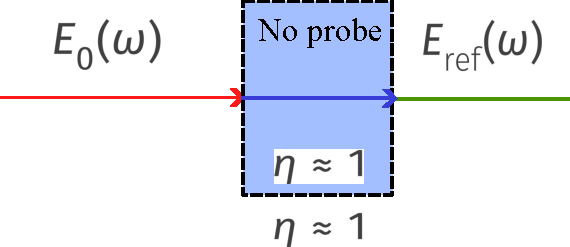
\includegraphics[width=0.5\textwidth]{images/reference.pdf}
  \end{center}
\end{frame}

\section{Complex transfer function}
\begin{frame}{Complex transfer function}
  With the transfered wave $E_\text{t}(\omega)$ and the reference wave $E_\text{ref}(\omega)$ a complex transfer function 
  \begin{equation}
    H_0(\omega) = \frac{E_\text{t}(\omega)}{E_\text{ref}(\omega)}
  \end{equation}
  can be defined.
  After plugging in the definitions of $E_\text{t}(\omega)$ and $E_\text{ref}(\omega)$, $H_0(\omega)$ yields
  \begin{equation}
    H_0 (\omega) = \frac{4 n_s(\omega)}{(n_s(\omega) +1)^2} \symup{exp}\left[-\kappa(\omega) \frac{\omega l }{c}\right] \symup{exp}\left[-i (n_s (\omega) - 1) \frac{\omega l}{c}\right]
  \end{equation}
  \end{frame}

\begin{frame}{Extracting phase}
  As the complex refractive index inside the exponent of $H_0(\omega)$ is rather tricky to solve it is assumed that the complex refractive index is similar to its real part $n_s(\omega) \approx n(\omega)$.
  This simplifies to 
  \begin{equation}
    H(\omega) = \frac{4n(\omega)}{(n(\omega) + 1)^2} \symup{exp}\left[-\kappa(\omega) \frac{\omega l }{c}\right] \symup{exp}\left[- i(n(\omega) - 1) \frac{\omega l}{c}\right]
  \end{equation}
  of which the phase information is
  \begin{equation}
    \Phi(H(\omega)) = -[n(\omega) - 1] \frac{\omega l}{c}
  \end{equation}
  and the logarithm is
  \begin{equation}
    \symup{ln}|H(\omega)| = \symup{ln}\left[ \frac{4n(\omega)}{(n(\omega) +1)^2}\right] - \kappa(\omega) \frac{\omega l}{c} \, .
  \end{equation}
\end{frame}

\begin{frame}{Determining the refractive index}
  With the phase information and logarithm it is now possible to determine the real refractive index 
  \begin{equation}
    n(\omega) = 1 - \frac{c}{\omega l} \Phi(H(\omega))
  \end{equation}
  and the complex refractive index 
  \begin{equation}
    \kappa(\omega) = \frac{c}{\omega l } \left( \symup{ln}\left[ \frac{4 n(\omega)}{(n(\omega) + 1)^2}\right] - \symup{ln}|H(\omega)|\right)
  \end{equation}
  from which the absorption coeffiecient
  \begin{equation}
    \alpha(\omega) = \frac{2 \omega \kappa(\omega)}{c}
  \end{equation}
  can be calculated.
  Note that a special unwrapping process is necessary to determine $\Phi(H(\omega))$, in python \textit{numpy.unwrap()} can be used to do this.
\end{frame}
\section{conclusion}
\begin{frame}{Refractive index}
  The refractive index can now be calculated by the formula defined in the beginning
  \begin{equation}
    n_s(\omega) = n - i \kappa \, .
  \end{equation}
  \newline
  \textcolor{tugreen}{conclusion:} This scheme gives an easy way to determine the refractive index of thick homogenous probes through time resolved THz-Spectroscopy.
  It can be extended to also take reflections inside the probe into account by using the Fabry-Perot factor in the transmitted wave.
  However, for most experimental setups this wont be necessary as the post-pulse is sufficiently delayed.

\end{frame}
\end{document} 